\titledquestion{Graph traversal}
Consider the following directed graph starting with A.

\centering
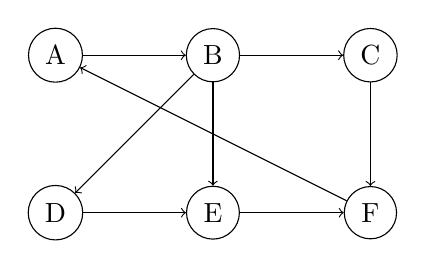
\begin{tikzpicture}[node distance=2cm]
    \node[circle, draw] (A) {A};
    \node[circle, draw, right of=A] (B) {B};
    \node[circle, draw, right of=B] (C) {C};
    \node[circle, draw, below of=A] (D) {D};
    \node[circle, draw, right of=D] (E) {E};
    \node[circle, draw, right of=E] (F) {F};

    \draw[->] (A) -- (B);
    \draw[->] (B) -- (C);
    \draw[->] (B) -- (D);
    \draw[->] (B) -- (E);
    \draw[->] (C) -- (F);
    \draw[->] (D) -- (E);
    \draw[->] (E) -- (F);
    \draw[->] (F) -- (A);
\end{tikzpicture}

\begin{parts}

\part[3]  Give the adjacency list for the graph. You should write the node in alphabetical order. (Leave it blank if the node has no neighbour)

\begin{align*} % Your solution here
    adj(A) =& [\underline{\qquad\qquad}],\\
    adj(B) =& [\underline{\qquad\qquad}],\\
    adj(C) =& [\underline{\qquad\qquad}],\\
    adj(D) =& [\underline{\qquad\qquad}],\\
    adj(E) =& [\underline{\qquad\qquad}],\\
    adj(F) =& [\underline{\qquad\qquad}],\\
\end{align*}


\part[3] Give the visited node order using the above adjacency list for Breadth First Search.
\begin{solution}
    
\end{solution}

\part[3] Give the visited node order using the above adjacency list for Depth First Search.
\begin{solution}
    
\end{solution}

\end{parts}